\documentclass[12pt]{article}

% Any percent sign marks a comment to the end of the line

% Every latex document starts with a documentclass declaration like this
% The option dvips allows for graphics, 12pt is the font size, and article
%   is the style

\usepackage[pdftex]{graphicx}
\usepackage{amsfonts}
\usepackage{amsmath}
\DeclareMathOperator*{\max_bottom}{max}
\usepackage{url}
\usepackage{hyperref}

\usepackage{caption}
\usepackage{subcaption}

\usepackage{graphicx}
\usepackage{amsmath}
\usepackage{adjustbox}
\usepackage{listings}

\lstset{language=python}

\hypersetup{
    colorlinks=true,
    linkcolor=blue,
    filecolor=magenta,      
    urlcolor=cyan,
    pdftitle={Sharelatex Example},
    bookmarks=true,
    pdfpagemode=FullScreen,
}


\usepackage{graphicx}
\graphicspath{ {./images/} }

% These are additional packages for "pdflatex", graphics, and to include
% hyperlinks inside a document.

\setlength{\oddsidemargin}{0.5cm}
\setlength{\evensidemargin}{0.5cm}
\setlength{\topmargin}{-1.6cm}
\setlength{\leftmargin}{0.5cm}
\setlength{\rightmargin}{0.5cm}
\setlength{\textheight}{24.00cm} 
\setlength{\textwidth}{15.00cm}
\parindent 0pt
\parskip 5pt
\pagestyle{plain}

% These force using more of the margins that is the default style
\newcommand{\namelistlabel}[1]{\mbox{#1}\hfil}
\newenvironment{namelist}[1]{%1
\begin{list}{}
    {
        \let\makelabel\namelistlabel
        \settowidth{\labelwidth}{#1}
        \setlength{\leftmargin}{1.1\labelwidth}
    }
  }{%1
\end{list}}


\begin{document}
\title{\Huge Introduction to machine learning - Homework 3}

\author{
  \textbf{Uri Kirstein}\\
  311137095 \\ sukirstn@campus.technion.ac.il
  \\ \\
  \textbf{Pavel Rastopchin}\\
  321082026 \\ pavelr@campus.technion.ac.il
  \\ \\ 
}

\maketitle


%\newpage
\section{Process and significant decisions}
\subsection{Automatic model selection}
As a part of non-mandatory assignment, we will implement the automatic model selection as an integral part of the mandatory assignment. For such task, we encapsulated all model evaluation scripts in one class called $modelSelector()$ (in short - Selector). As we have 3 prediction tasks, the Selector will train all candidate models on training set, and test all of them on the validation set. The difference between the tasks is that different performance metrics will be used. At the end of validation, each model will get a score for it's performance for each prediction task.

\subsection{Different models for different tasks}
As it stated in the assignment document -  "one size doesn't fit all", i.e. different models can be the best models for each task. To handle this, we decided to include in our $modelSelector()$ class an option to select best model for each task. At the time of writing this paragraph we still don't know if the same model will be selected for all tasks or not.

\section{Data Preparation}
\subsection{First adjustments}
At the end of exercise 2 the data preparation process was:
\begin{enumerate}
\item Delete illogical values (i.e. negative average monthly expenses)
\item Fill missing values via linear regression with another highly correlated features. We impute from the highest to lowest correlated feature by absolute value in descending order, and we stop when correlation drops below 0.8.
\item For each feature, delete values that are three standard deviations from the norm
\item Again fill missing values via linear regression
\item Again delete illogical values
\item Delete features that were only used for linear regression
\item Fill the remaining missing numerical values as the mean value of that feature
\item Categorical features are filled by the same distribution as the rest of the values in this categorical feature.
\end{enumerate}

Imputation is done on all three sets. All statistics were computed on the train set only. As can be seen, for our process we use only the target features
and features that are highly ($\geq 0.8$) correlated with them.\\

\begin{adjustbox}{max width=\linewidth}
\begin{lstlisting}
NUMERIC_TARGET_FEATURES = ['Avg_environmental_importance', 'Avg_government_satisfaction',
                           'Avg_education_importance', 'Avg_monthly_expense_on_pets_or_plants',
                           'Avg_Residancy_Altitude', 'Number_of_valued_Kneset_members',
                           'Yearly_ExpensesK', 'Weighted_education_rank']
CATEGORIC_TARGET_FEATURES = ['Most_Important_Issue']
\end{lstlisting}
\end{adjustbox}\\\\


The highly correlated features are:\\

\begin{adjustbox}{max width=\linewidth}
\begin{lstlisting}
NUMERIC_USEFUL_FEATURES = ['Avg_Residancy_Altitude', 'Avg_Satisfaction_with_previous_vote',
                           'Avg_education_importance', 'Avg_environmental_importance',
                           'Avg_government_satisfaction', 'Avg_monthly_expense_on_pets_or_plants',
                           'Avg_monthly_expense_when_under_age_21', 'Avg_monthly_household_cost',
                           'Avg_monthly_income_all_years', 'Avg_size_per_room', 'Last_school_grades',
                           'Number_of_valued_Kneset_members', 'Phone_minutes_10_years',
                           'Political_interest_Total_Score', 'Weighted_education_rank',
                           'Yearly_ExpensesK']
\end{lstlisting}
\end{adjustbox}\\

This list, together with our categorical feature 'Most\_Important\_Issue' and the label 'Vote' are all the features used in the data preparation process. Every other feature was discarded at the very first step.\\
For the scaling step we had to find the distributions of the features we haven't chosen in part 2. Again, we divided them to two groups - gaussian features, which will be z-score normalized, and non-gaussian features, which will be min-max normalized to $[1, -1]$. Features that were not close to uniform distribution were grouped with the gaussian features. By drawing the distributions we found that:\\

\begin{adjustbox}{max width=\linewidth}
\begin{lstlisting}
    gaussian_features = ['Avg_Residancy_Altitude', 'Avg_education_importance', 'Avg_environmental_importance',
                         'Avg_government_satisfaction', 'Number_of_valued_Kneset_members']
    non_gaussian_features = ['Avg_monthly_expense_on_pets_or_plants', 'Weighted_education_rank',
                             'Yearly_ExpensesK']
\end{lstlisting}
\end{adjustbox}\\

\subsection{Using the validation set}
After checking the model outputs of the latter parts of this exercise, we have found we have much inferior results between the training set (accuracy $>90\%$) and the validation and train sets (accuracy $\approx 75\%$). 
After discussing with the TA in charge of the course and talking to colleagues in class, we realized this behaviour is odd. In an attempt to fix it we decided to use the validation data in all parts of our pre-processing, so we can have a more stable statistical confidence. We expect that the accuracy dropoff, at least between the train and validation sets, will be much smaller.

\section{Implementing feedback on Homework 2}
It was roughly at this stage when we got the feedback on HW2. We've implemented the suggested changes.
\subsection{Noise, Outliers and Imputation}
As suggested, we will only build a linear regression model for features with $|correlation| \geq  0.93$. This means we can discard even more features in our very initial step. The remaining correlated features are:\\

\begin{adjustbox}{max width=\linewidth}
\begin{lstlisting}
CORRELATED_NUMERIC_FEATURES = ['Avg_Satisfaction_with_previous_vote',
                               'Avg_monthly_expense_when_under_age_21', 'Avg_monthly_household_cost',
                               'Avg_size_per_room', 'Phone_minutes_10_years']
\end{lstlisting}
\end{adjustbox}\\
\\

We now delete values that are three standard deviations or more from the mean of the feature only from the features that are gaussian.

\subsection{Fill missing categrical features}
Previously we have just sampled labels from the same distribution of that feature as seen on the train and validation sets. As suggested, we are using a classifier to try and predict the missing values. The chosen classifier is a KNN classifier $K=10$.\\
We had changed the order of actions, as the KNN model is sensitive to data scaling and normalization. The new order of actions is:
\begin{enumerate}
\item Fill missing numeric values
\item Scale and normalize numeric values
\item Fill categoric values
\end{enumerate}

\section{Candidate models}
In this section we discuss the candidate models which were selected for our experiments. For the task of most probable voters, we need to predict probabilities, but not the exact tag, so we want to use models which can provide this functionality. Based on post in \href{https://www.researchgate.net/post/What_are_the_best_supervised_classifiers_to_classify_the_problem_of_multiclass_classification}{www.researchgate.net} stating that SVM, KNN and Random Forest can successfully handle a problem of multi-class classification, we decided to choose those two models in addition to MLP, resulting a total of four candidate models.

\subsection{Hyper parameters tuning with k-fold cross validation}
In order to select the best model candidates, we need to perform 5-fold cross validation using training set only. The cross validation process for all models implemented in $crossValidator$ class. In all our cross-validation experiments we used the $f1_score$ as model performance measurement. While its not the same measurement we selected for each task, it's a stricter requirement than all other metrics we will describe in the following sections.

\subsection{Support vector machine hyper-parameters tuning}
Based on a post in \href{https://www.researchgate.net/post/Is_it_necessary_to_choose_kernels_in_SVM_according_to_application}{www.researchgate.net} the most important parameters for SVM are the kernel and the C parameter. Kernel determines the shape of separating hyper-plane and C parameter responsible for its complexity. A larger C makes the model more complex and lowers its bias, hence increasing chance of over-fitting. A low C gives a model with low variance and high bias. As we could not achieve convergence with linear kernel, we will use SVM with RBF kernel. To select the right value for the C hyper parameter we used the k-fold cross validation technique. First we performed cross-validation of a big range of C values with exponential steps and plotted it. Then we repeated the process with a smaller range and smaller steps for fine tuning. As we can see from the plots, the best accuracy was achieved with $C=20$ after which we can't see any improvement, thus this value with be selected for SVM model.

\begin{figure}[h]
\centering
\begin{subfigure}{.5\textwidth}
  \centering
  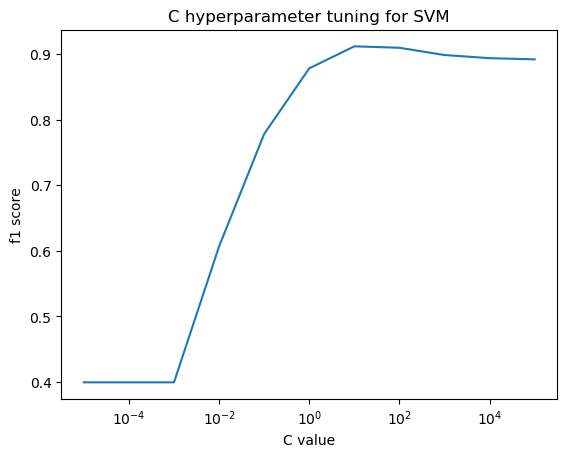
\includegraphics[width=.6\linewidth]{Cross_valid_plots/SVM_C_hyper_fig_coarse.png}
  \caption{C coarse tuning}
  \label{fig:sub1}
\end{subfigure}%
\begin{subfigure}{.5\textwidth}
  \centering
  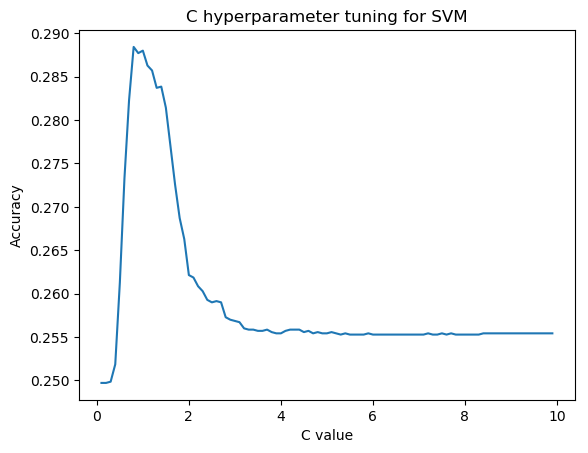
\includegraphics[width=.6\linewidth]{Cross_valid_plots/SVM_C_hyper_fig_fine.png}
  \caption{C fine tuning}
  \label{fig:sub2}
\end{subfigure}
\caption{C hyper parameter tuning}
\label{fig:test}
\end{figure}


\subsection{K nearest neighbours}
While using KNN, under some circumstances, it is better to weight the neighbors proportionally to the inverse of the distance from the query point. As we would like to experiment with both options, we will create two KNN classifiers with two different distance functions and test their performance. To select the right value for k hyper parameter we used the k-fold cross validation technique for both knn models. The optimal accuracy is $k=3$. Clearly, the KNN with weighted distances performed better for all values of k.
\begin{figure}[h]
\centering
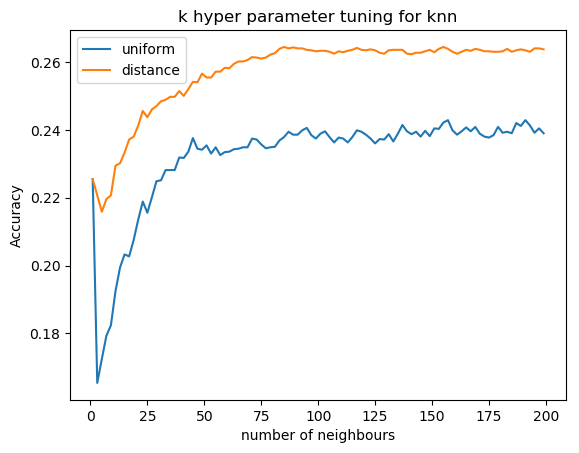
\includegraphics[width=0.4\textwidth]{Cross_valid_plots/k_hyper_fig}
\caption{k hyper parameter tuning}
\end{figure}

\subsection{Random Forest}
A random forest fits a number of decision tree classifiers on various sub-samples of the dataset and uses averaging to improve the predictive accuracy and reduce over-fitting. According to \href{https://medium.com/all-things-ai/in-depth-parameter-tuning-for-random-forest-d67bb7e920d}{medium.com post} the most important parameters of this classifier are:
\begin{enumerate}
	\item \textbf{Number of trees -} The higher the number of trees the better, but adding a lot of trees can slow down the training process. Based on the plots, 50 trees suffice as greater values don't improve the score.
	\item \textbf{Maximum depth -} Represents the depth of each tree in the forest. A deeper tree tends to overfit more. Based on the plots we decided to set the depth to 8 as bigger depths do not increase accuracy.
	\item \textbf{Minimum samples split -} represents the minimum number of samples required to split an internal tree node. As we can see on the plot, the best accuracy was achieved with the smallest value of 0.01 which means minimum 70 samples is required for a split.
\end{enumerate}

\begin{figure}[h]
\centering
\begin{subfigure}{0.3\textwidth}
  \centering
  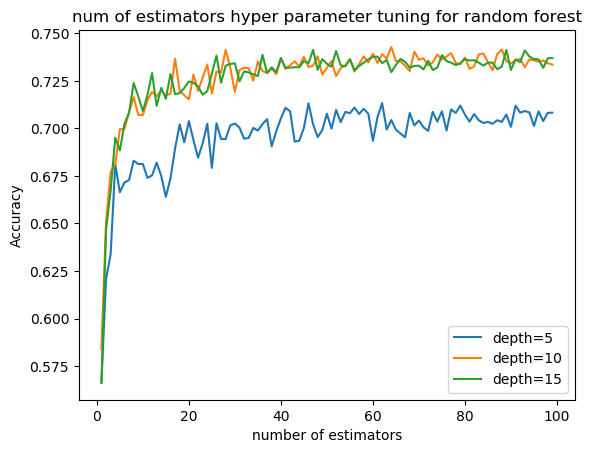
\includegraphics[width=1\linewidth]{Cross_valid_plots/n_hyper_forest_fig}
  \caption{n tuning}
  \label{fig:sub1}
\end{subfigure}%
\begin{subfigure}{0.3\textwidth}
  \centering
  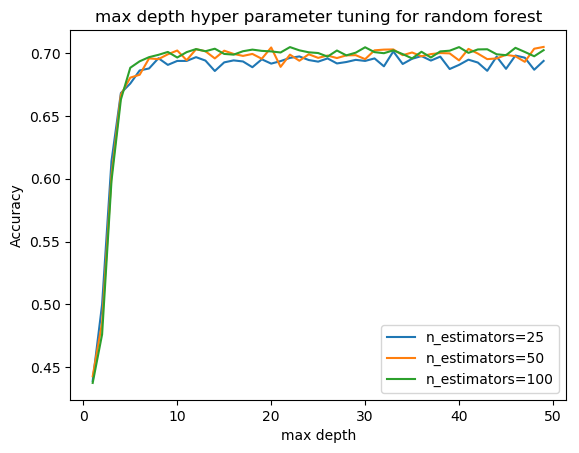
\includegraphics[width=1\linewidth]{Cross_valid_plots/d_hyper_forest_fig}
  \caption{depth tuning}
  \label{fig:sub1}
\end{subfigure}%
\begin{subfigure}{0.3\textwidth}
  \centering
  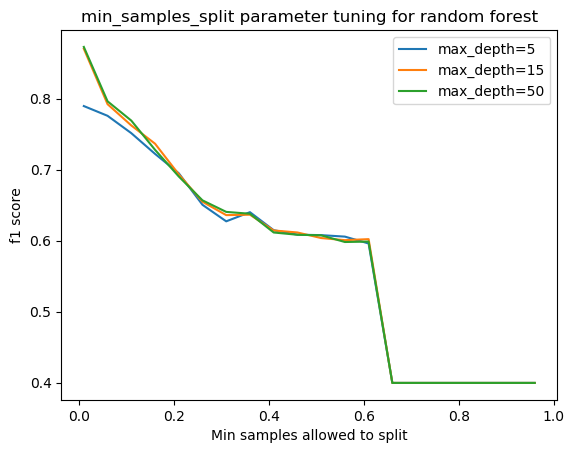
\includegraphics[width=1\linewidth]{Cross_valid_plots/s_hyper_forest_fig}
  \caption{split tuning}
  \label{fig:sub2}
\end{subfigure}
\caption{Random forest parameters tuning}
\label{fig:test}
\end{figure}

We have found other parameters less important (and less intuitive), thus for them we will use the default values.

\subsection{Multi-layer perceptron}
Multi-layer Perceptron classifier. This model optimizes the log-loss function using LBFGS or stochastic gradient descent. In this section we discuss the most important parameters of MLP and the values we have chosen. Our decisions were mostly based on the post in \href{https://stats.stackexchange.com/questions/181/how-to-choose-the-number-of-hidden-layers-and-nodes-in-a-feedforward-neural-netw}{stats.stackexchange.com}.
\begin{enumerate}
	\item \textbf{Number of hidden layers -} There is a consensus that one hidden layer is sufficient for the large majority of problems. We decided to test three options in the cross-validation process: 1, 2 and 3 hidden layers.
	\item \textbf{Hidden layer size -} There is rule of thumb for supervised learning problems. The upper bound on the number of hidden neurons that will not result in over-fitting is:
\begin{gather*}
N_h = \dfrac{N_s}{\alpha * (N_i + N_o)}
\end{gather*}
when $N_o$ is number of output neurons, $N_i$ is number of input neurons, $N_s$ number of training samples and $\alpha$ is an arbitrary factor between 2 and 10. In our case, for $\alpha = 10$ the upper bound is 166 neurons in the hidden layer. Thus, during cross validation we will test numbers up to this threshold.
	\item \textbf{Activation function -} we will test two options: ReLU and Tanh.
\end{enumerate}

\begin{figure}[h]
\centering
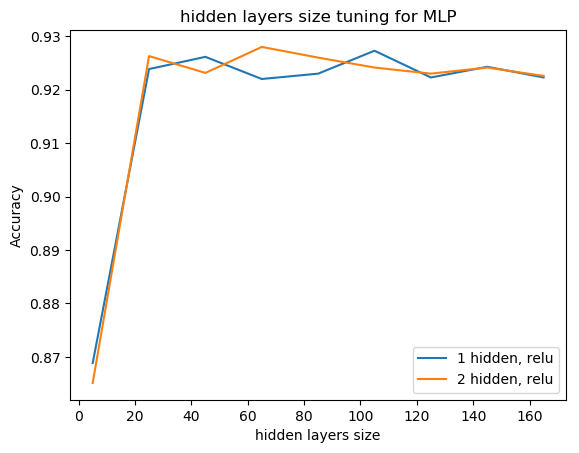
\includegraphics[width=0.4\textwidth]{Cross_valid_plots/mlp_h_fig}
\caption{MLP cross validation results}
\end{figure}

\newpage
\section{Performance measurements}
\subsection{Majority votes measurement}
For predicting which party will win the majority of the votes we propose using the most simple measurement that comes to mind - "binary score": if the majority of predicted tags are from the same class as in validation set, the model score is 1 and 0 otherwise. This method can give us multiple models which can predict the winner party. To make the method more selective we decided to use f1 score as a secondary measurement.

\subsection{Votes division measurement}
In this task we want to predict correctly the division of the total votes (in test set) between the parties, but not individual votes. In other words, we want to compare a histogram of predicted votes to the histogram of true votes in the test set, thus the metrics we use is an Euclidean distance between two histograms:
\begin{gather*}
D = \sqrt[2]{\sum_{i=0}^{12} (histPredicted_i - histTrue_i)^2}   
\end{gather*}
According to this measurement, a predicted votes distribution histogram which is very different form the true histogram will be "far away" (in terms of Euclidean distance) from it. On the other hand, if the predicted votes distribution histogram is similar to the true histogram, they will have a small distance. Thus, the model with the shortest Euclidean distance will be considered the best model for this task.

\subsection{Most probable voters measurement}
In this task we should predict the probability of each voter to vote for each party, but not the exact label. That's why the first approach was to use custom metrics for this task. Denoting $P_i$ as set of predicted voters whose probably to vote $i$ party is above $threshold$, $T_i$ as true set of voters for $i$ party, we can state the following:
\begin{enumerate}
	\item $P_i \cap T_i$ is the actual amount of voters which will be provided transportation. Generally speaking, a large intersection is good, thus it will increase the score.
	\item $P_i - T_i$ are the mispredicted voters, which will not vote for the given party, but will get a free ride. Of course that a large $P-T$ is bad, thus it will decrease the score.
	\item $T_i - P_i$ - are actual voters which will not get a transportation and maybe will not vote at all as a result. big $T-P$ is bad, thus it will decrease the score.
\end{enumerate} 
Finally we ended up with following score calculation:\\
\begin{gather*}   
   Score = \sum_{i=0}^{12} |P_i \cap T_i|-|P_i - T_i|-|T_i -P_i|  
\end{gather*}
During our work on this prediction task we noticed that weighted f1 score perfectly corresponds to our custom score. As a result we decided to use weighted f1 score as a measurement for this prediction task. 


\section{Prediction results and chosen model}
In this section we will discuss the results of each prediction task, the quality of the results according to the measurements and which model was selected for each prediction task.
\subsection{Majority votes}
To visualize the prediction results on validation set we will show the histogram of true labels of validation set and of predicted labels. According to the plots, 3 models predicted the winner correctly, but the MLP model got the highest f1 score, thus it was selected automatically as the best model for this task.

\begin{figure}[htp]
\centering
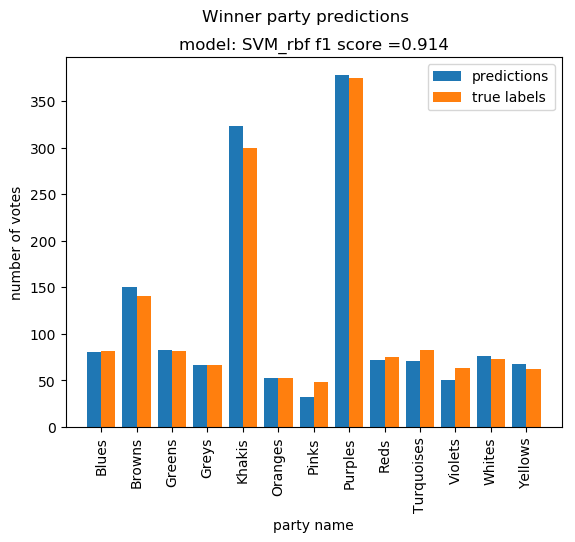
\includegraphics[width=.4\textwidth]{Winner_party_plots/SVM_rbf_fig}
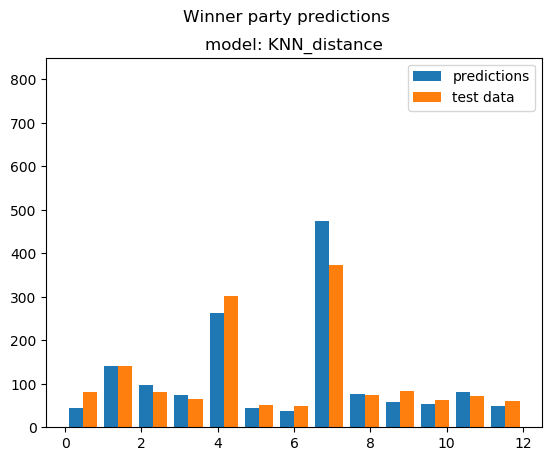
\includegraphics[width=.4\textwidth]{Winner_party_plots/KNN_distance_fig}
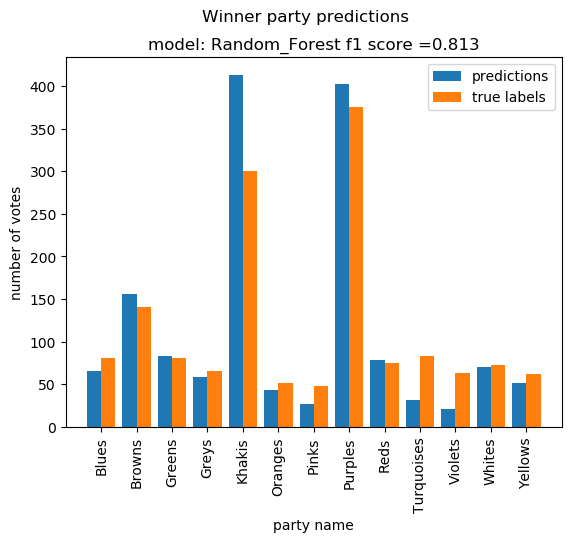
\includegraphics[width=.4\textwidth]{Winner_party_plots/Random_Forest_fig}
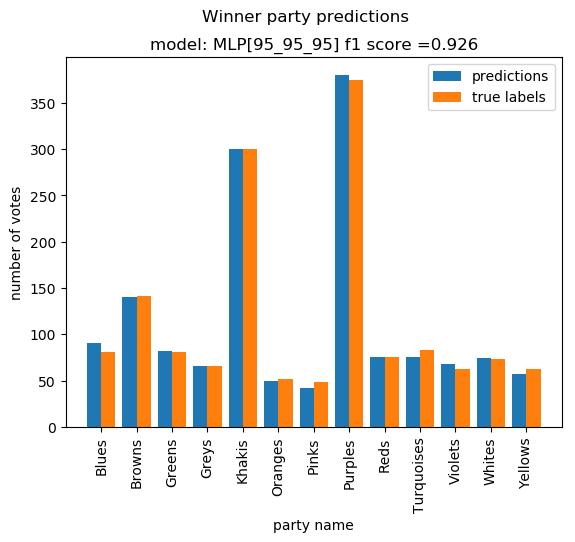
\includegraphics[width=.4\textwidth]{Winner_party_plots/MLP[95_95_95]_fig}
\end{figure}

\newpage
\subsection{Votes division}
To visualize the prediction results on validation set we will use histogram of true labels of the validation set and of predicted labels. According to the metrics we chose for this task, we are interested in the model which achieved the smallest Euclidean distance between the histograms. As stated in previous sections, the most similar histograms have the smallest euclidean distance. In conclusion, MLP classifier achieved best performance on the validation set with a final score of 16. 

\begin{figure}[htp]
\centering
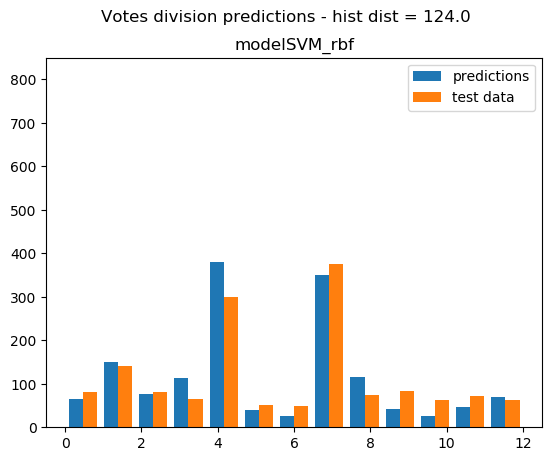
\includegraphics[width=.4\textwidth]{Division_prediction_plots/SVM_rbf_fig}\quad
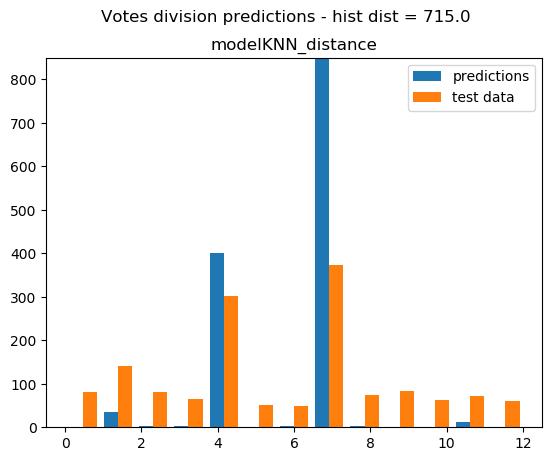
\includegraphics[width=.4\textwidth]{Division_prediction_plots/KNN_distance_fig}\quad
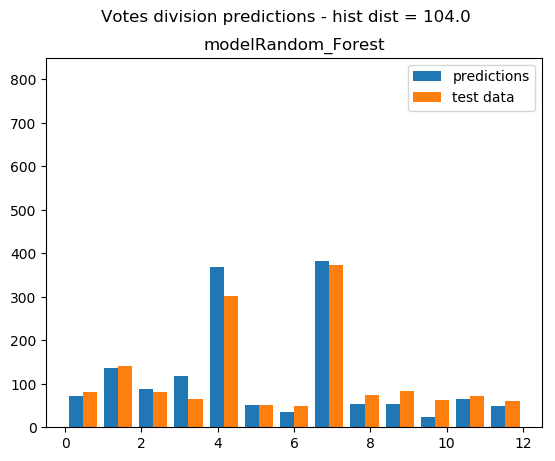
\includegraphics[width=.4\textwidth]{Division_prediction_plots/Random_Forest_fig}
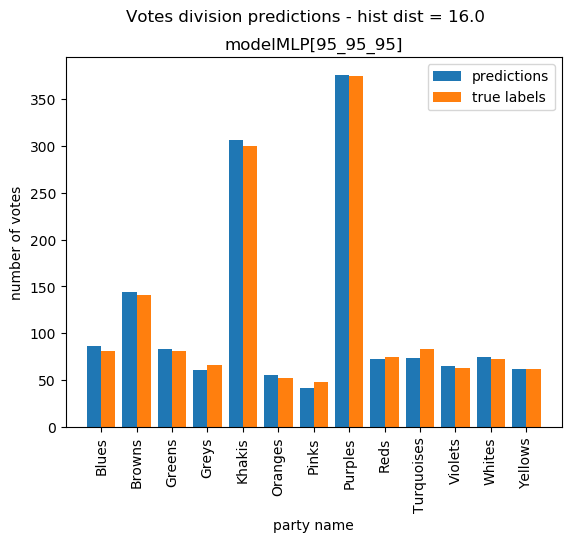
\includegraphics[width=.4\textwidth]{Division_prediction_plots/MLP[95_95_95]_fig}
\end{figure}


\subsection{Voters transportation}
To visualize the prediction results on validation set we will use bar charts. Each color represents a set of one type, and the bar height represents the size of the set. The grey color represents "forgotten" voters, i.e. the voters who are willing to vote for a given party, but have not been provided transportation. The red color is a sets of votes who are not voting for the party but still got a free ride. The green bar represents the voters which will vote and actually get transportation. The grey and the red bars' heights effect negatively on the score, while the green bar's height effects it positively. As we can see, Random Forest has a very low performance score, which means according to its probability predictions the parties will not provide transportation to their potential voters or will give a free ride to people who don't want to vote for them. On the other hand, MLP was much more accurate with it's probability predictions and provided each party a relatively large list of true potential voters. For visualization, a person was added to the party's list only if he will vote to this party with a probability higher than $0.5$. Our implementation provides the functionality the set the probability threshold which will maybe change the list of predicted votes ?????????????????????????????????????????????????????????, but not change the model, as it's been selected according to f1 score. 

\begin{figure}[h]
\centering
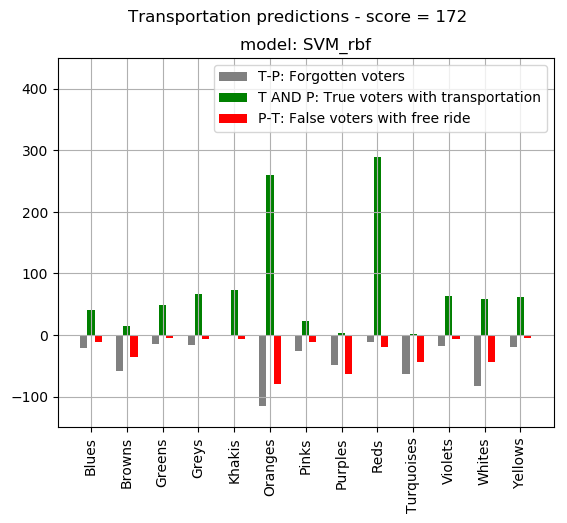
\includegraphics[width=.4\linewidth]{Vote_prediction_plots/SVM_rbf_fig.png}
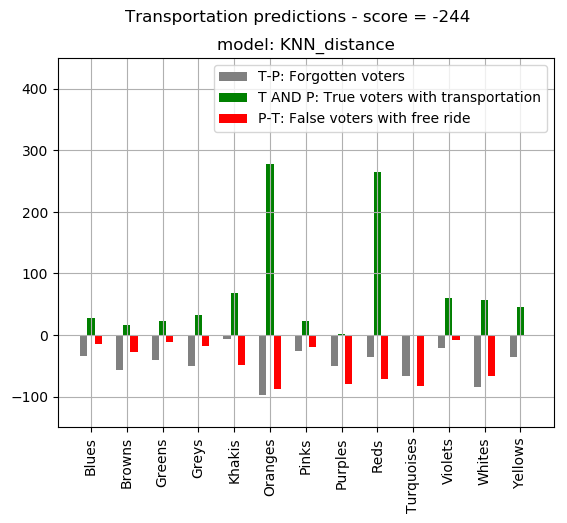
\includegraphics[width=.4\linewidth]{Vote_prediction_plots/KNN_distance_fig}
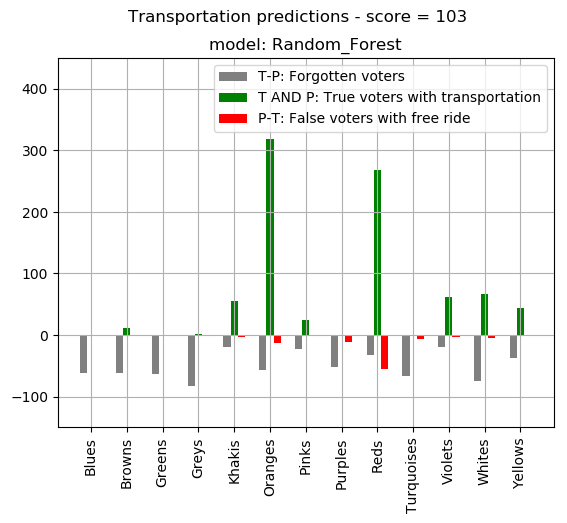
\includegraphics[width=.4\linewidth]{Vote_prediction_plots/Random_Forest_fig}
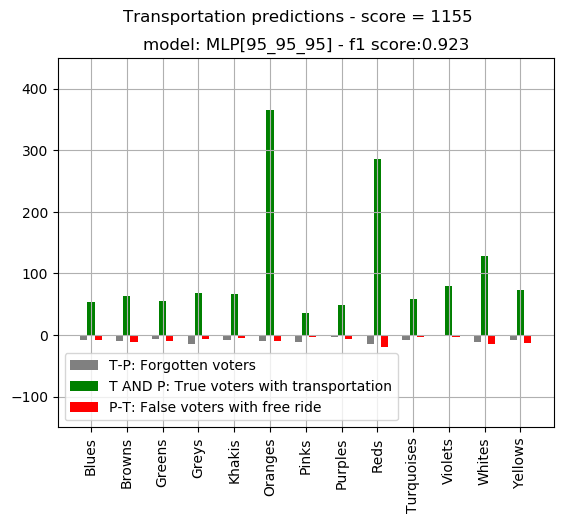
\includegraphics[width=.4\linewidth]{Vote_prediction_plots/MLP[95_95_95]_fig}
\caption{Models performance for transportation task}
\label{fig:test}
\end{figure}


\section{Final answers}
The best models are:

\small
\begin{verbatim}
best model for transportation is  MLP[95_95_95]
best model for winner prediction is  MLP[95_95_95]
best model for vote division is  MLP[95_95_95]
\end{verbatim}
\normalsize


\subsection{Which party will win}
As described previously, the best model for this task is SVM with RBF kernel, and its final prediction was:
\small
\begin{verbatim}
MLP[95_95_95]  prediction -  Purples  party will win the elections.
\end{verbatim}
\normalsize

\subsection{Votes division}
As described previously, the best model for this task is Random Forest, and its final prediction was:
\small
\begin{verbatim}
MLP[95_95_95]  prediction - Vote division:
Party  Blues : 5.6 %
Party  Browns : 9.0 %
Party  Greens : 5.5 %
Party  Greys : 4.5 %
Party  Khakis : 21.0 %
Party  Oranges : 2.9 %
Party  Pinks : 3.2 %
Party  Purples : 25.0 %
Party  Reds : 5.1 %
Party  Turquoises : 5.3 %
Party  Violets : 3.3 %
Party  Whites : 5.2 %
Party  Yellows : 4.3 %
\end{verbatim}
\normalsize

\subsection{Confusion matrix and test error}
\begin{figure}[htp]
\centering
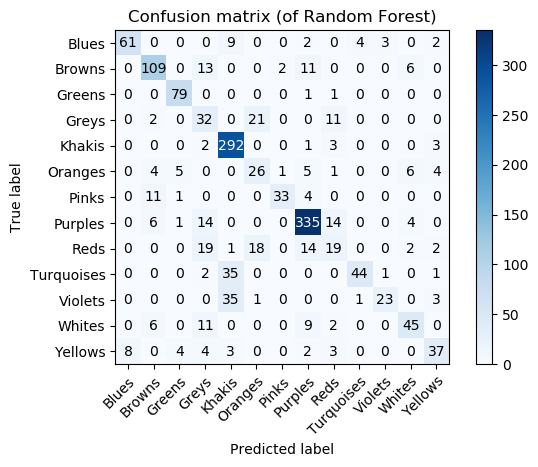
\includegraphics[width=0.5\textwidth]{confusion_matrix/confusion_fig}
\caption{Confusion matrix of MLP}
\end{figure}

\begin{verbatim}
Model  MLP[95_95_95]  reached  6.4 % error.
\end{verbatim}

\newpage
\section{Comparison with one model approach}
In addition to the "different model for each task" selection we want to try the "one model" approach. In this section we will answer the same questions as in our prediction tasks, add a confusion matrix and test error result.
\subsection{How do we select the best model}
We decided to create automatic model selection process in the same class $modelSelector$ which selects one model for all tasks by executing a two stage process:
\begin{enumerate}
\item Evaluate all candidate models on validation set and select all the models which predicted correctly the winner party. We see this task as the most important as it predicts who is the winner - the most important outcome of the elections.
\item Evaluate all selected models on validation set to predict the most probable voters for the transportation task, and select the model which performed better than others according to metrics of this task. We see the transportation task as the second most important task for its serious financial implications. Finally, the model with best performance was selected for all tasks. 
\end{enumerate}
We don't evaluate the model on the validation set to get a score for the votes division task, as wee see this task as the least important. Moreover, as we can see from our previous results, a model with best transportation task score, actually handles very well the vote division task. Our model of choice is MLP. As we saw in previous section, this model was selected for each prediction task independently, so the final results are exactly the same.  

\subsection{Comparison}
As we can see, in both cases we achieved the same results as the same model was selected.
\begin{enumerate}
\item The main advantage of one for all method is simplicity of implementation.
\item In our case the same model was selected for all three tasks, which is not necessarily always true. If there are different models which are best for different task, we are giving up on performance while selecting only one model for all tasks.
\end{enumerate}

\section{Feature manipulation - Bonus Assignment}
In this section we look for features which can be manipulated to cause another party to win. To complete this task we've created a class $featureManipulator$ that automatically finds such features. First, we provide the class the best model for winner party prediction. Them, in iterative manner, Feature Manipulator decreases or increases one column of the validation or test data one by one, by a given constant $C$. In each iteration we start with relatively small values of $C$ and increase them gradually, until the model predicts another party as a winner. To visualize it we plot the histograms of original predictions, new predictions on altered data and true labels.   

\begin{figure}[ht]
	\centering
	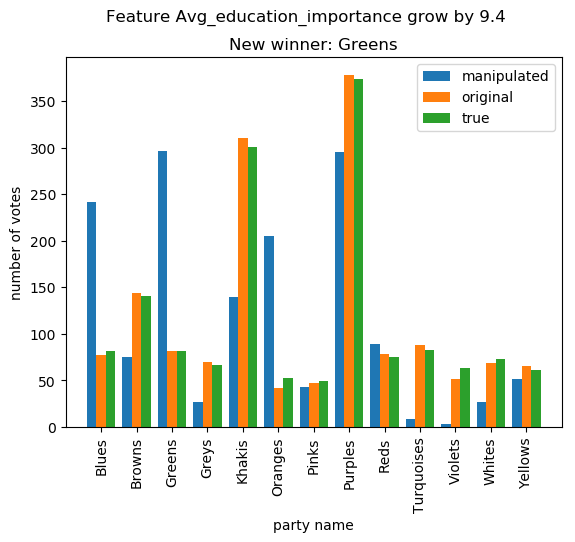
\includegraphics[width=0.2\textwidth]{dramatic_feature/Avg_education_importance_increased}
	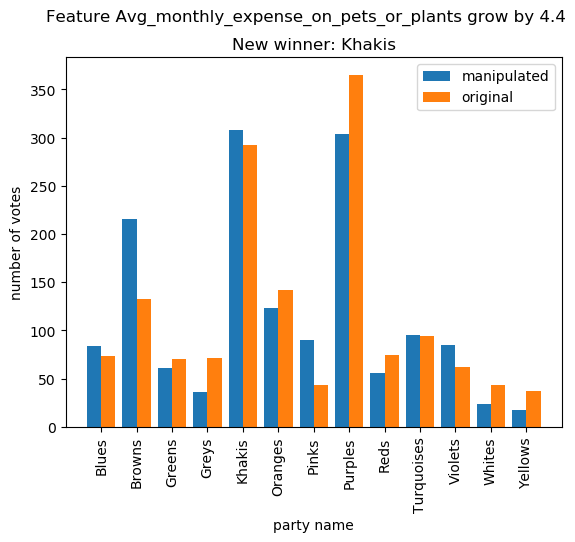
\includegraphics[width=0.2\textwidth]{dramatic_feature/Avg_monthly_expense_on_pets_or_plants_increased}
	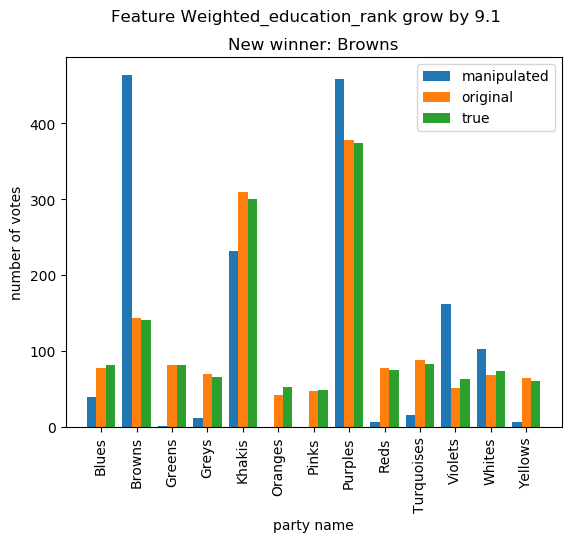
\includegraphics[width=0.2\textwidth]{dramatic_feature/Weighted_education_rank_increased}	
	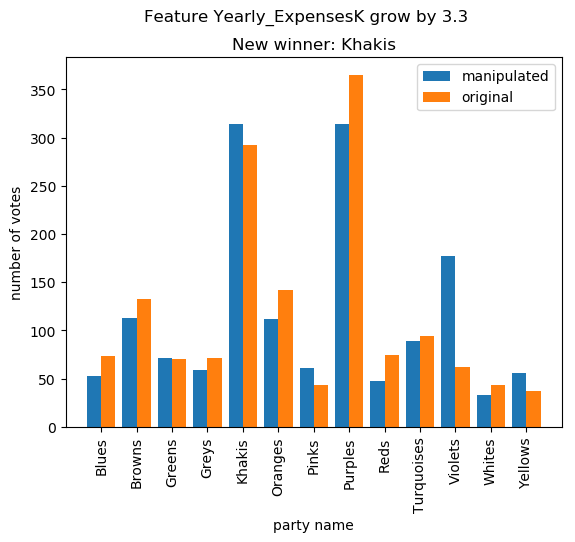
\includegraphics[width=0.2\textwidth]{dramatic_feature/Yearly_ExpensesK_increased}					
\end{figure}

To summarize the results:

\begin{enumerate}

\item If \textit{Weighted education rank} grows by 9.1 the Browns will win

\item If \textit{Avg environmental importance} grows by 5.8 the Blues will win

\item If \textit{Avg education importance} growa by 9.4 the  Greens will win

\item If \textit{Avg monthly expense on pets or plants} grows by 11.3 the Yellows will win

\item If \textit{Yearly Expenses K} grows by 2.9 the Khakis will win

\end{enumerate}

\newpage
\section{Widrow-Hoff}
In this section we implement Adaline algorithm. First we implemented iterative Adaline which worked properly but was extremely slow. Thus the best option is an analytic solution which we implemented as well. Then we implemented a 1-vs-all technique in $Adaline$ class for multiclass classification. i.e. for the Iris dataset we trained automatically 3 Adaline binary classifiers, and 10 classifiers for Digits dataset.
\subsection{Results on Iris and Digits datasets}
We used the code from \textit{"Comparing various online solvers"} to generate the plots. Those plot were generated using our $Adaline$ class which includes a proper number of Adaline classifiers, depending on number of classes, which makes it a multiclass classifier. 
\begin{figure}[ht]
	\centering
	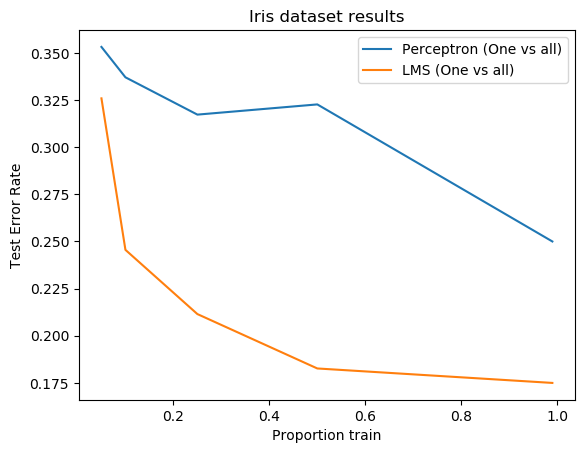
\includegraphics[width=0.4\textwidth]{weirdo_hoff_plots/iris}
	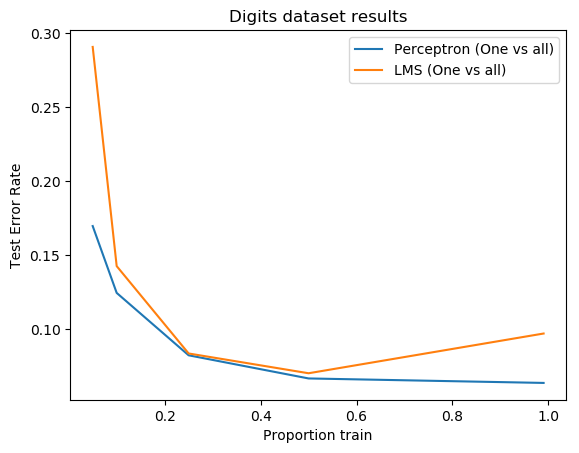
\includegraphics[width=0.4\textwidth]{weirdo_hoff_plots/digits}			
\end{figure}

\subsection{Results on generated datasets}
We used the same technique to compare two models as in the previous section. 
\begin{figure}[ht]
	\centering
	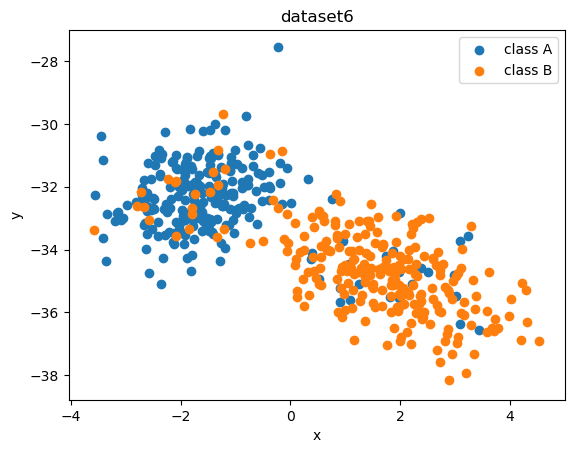
\includegraphics[width=0.4\textwidth]{weirdo_hoff_plots/dataset_lms}
	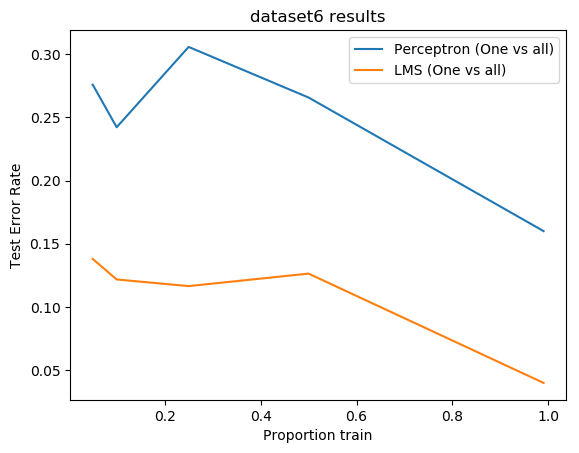
\includegraphics[width=0.4\textwidth]{weirdo_hoff_plots/plot_lms}
	\caption{LMS perform better on a noisy dataset}
\end{figure}
As we can see, LMS requires a much smaller train set, i.e. converge faster in terms of number of samples. The dataset that we chose is a linearly non-separable dataset as a result of random noise. The explanation is that noisy samples don't affect much the separation line of LMS algorithm, as their portion of the dataset is rather small. On the other hand, they do affect the Perceptron, because if the datasets are not linearly separable, we can't be sure that it will converge at all. 

\begin{figure}[ht]
	\centering
	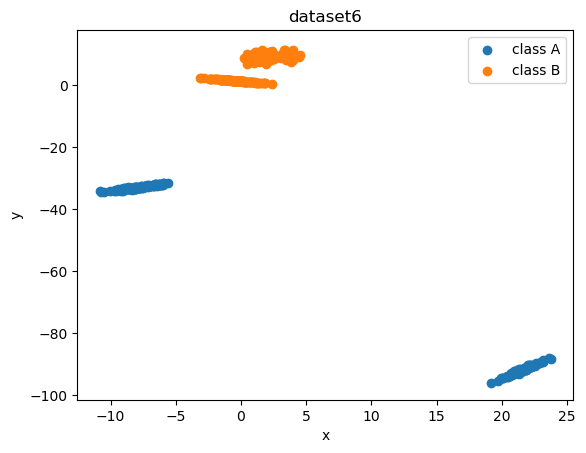
\includegraphics[width=0.4\textwidth]{weirdo_hoff_plots/dataset_perc}
	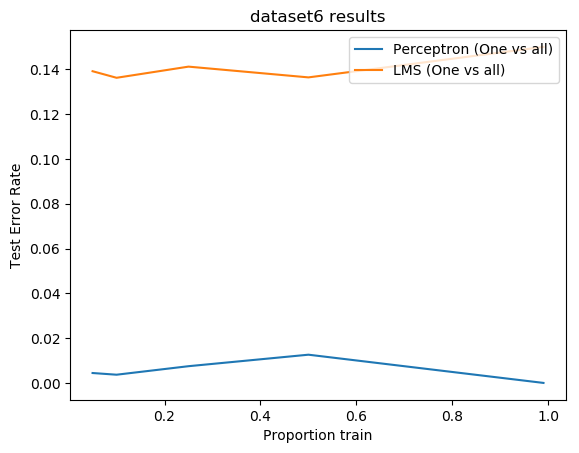
\includegraphics[width=0.4\textwidth]{weirdo_hoff_plots/plot_perc}
	\caption{Perceptron perform better on a well-separated datasets without noise}			
\end{figure}
In this example we have very compact clusters which are linearly separable, a small portion of the data set suffices for the convergence of the Perceptron.


\end{document}
